\section{Contract languages}
\label{languages}

Figure \ref{fig:languagediagram} gives an overview of smart contract languages.
Smart contracts are a comparably new discipline.
Hence, early platforms offering smart contracts, like Ethereum, are using a direct compilation into the target low-level language as presented in (B)~\cite{Ethereum2018Vyper}.
The approach in (A) utilises intermediary representations to allow program optimisation and verification. 
Among the projects that follow this approach is Tezos with Liquidity~\cite{OCamlProSAS2018} and Michelson~\cite{DynamicLedgerSolutions2017}. 
Likewise, Scilla is an IR that is targeted by more general languages and compiles down to be executed on a distributed VM~\cite{Sergey2018}.
Ethereum is in the process of adopting this approach with Yul~\cite{EthereumFoundation2018IULIA}.
Last, some projects, like Bitcoin~\cite{BitcoinWiki2018Script}, typically use scripts directly written in the low-level stack-based language.



%\dha{For process (A) probably use Tezos or something like that that have a high-level language, IR and low-level lang.}

\begin{figure}[!t]
\normalsize
\centering
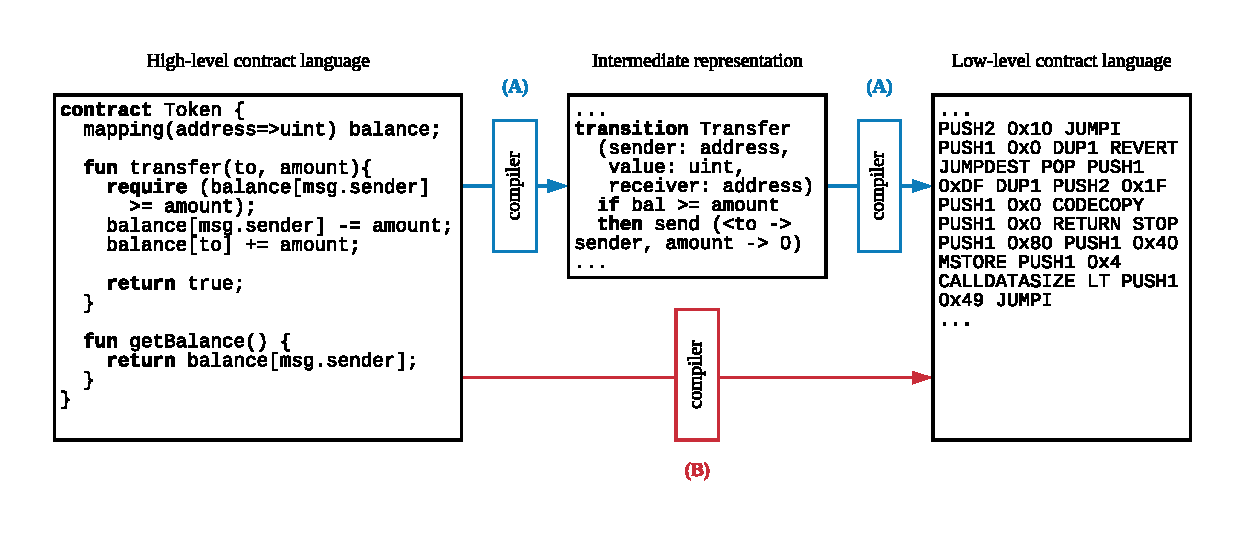
\includegraphics[width=\columnwidth]{fig/Language.pdf}
\caption{Different abstraction levels of smart contract languages. (A) represents an approach of compiling high-level languages through a intermediary representation (IR) to a low-level language. The contract can be verified and optimised at the IR level. These verification methods and optimisations can then be used for multiple high-level languages. (B) represents the direct compilation from a high-level language to a low-level representation. This approach requires only a single compiler and is thus faster to implement.}
\label{fig:languagediagram}
\end{figure}


\subsection{Overview}
The overview we present in table \ref{tab:high-level} is based on five different criteria as listed below. The table gives a general overview. We explain the security properties of the languages within the following subsections.
\begin{itemize}
\item \emph{Type}: We differentiate between high-level, IR, and low-level languages.
\item \emph{Paradigm}: This describes the main paradigm of the language. Note that most languages support multiple paradigms and this criterion is more of an indication of the prevalent paradigm.
\item \emph{Instructions}: The possible instruction set that a language supports can be restricted or Turing-complete.
\item \emph{Semantics}: Languages have a formal or informal semantic. Formal semantics define the exact behaviour of programs written in that language. Informal semantics mostly let the compiler define the exact behaviour.
\item \emph{Metering}: Smart contracts executed on a distributed ledger are re-executed by several nodes. As these computations are costly, metering is a way to charge and limit the execution of a program.
\end{itemize}
\begin{table*}[h]
\centering
\caption{Overview of languages for smart contracts.}
\label{tab:high-level}
\begin{tabularx}{\textwidth}{XXXXXr}
\toprule
\textbf{Language} & \textbf{Paradigm} & \textbf{Instructions} & \textbf{Semantics} & \textbf{Metering} & \textbf{Ref.} \\ \toprule
\textit{Solidity} & object-oriented & Turing-complete & informal\textsuperscript{\dag} & gas, limit & \cite{Ethereum2018Solidity} \\
\textit{Vyper} & procedural & restricted & informal\textsuperscript{\dag} & gas, limit & \cite{Ethereum2018Vyper} \\
\textit{Bamboo} & procedural & Turing-complete & semi\textsuperscript{\dag} & gas, limit & \cite{Hirai2018Bamboo} \\
\textit{Flint} & procedural & Turing-complete & informal & gas, limit & \cite{Schrans2018} \\
\textit{Pyramid Scheme} & functional & Turing-complete & informal & gas, limit & \cite{Burge2018} \\
\textit{Obsidian} & object-oriented & -- & informal & -- & \cite{Coblenz2017} \\
\textit{Rholang} & concurrent & Turing-complete & informal & phlogiston & \cite{Meredith2018} \\
\textit{Liquidity} & functional & restricted & semi\textsuperscript{\dag} & gas, limit & \cite{OCamlProSAS2018} \\
\textit{DAML} & functional & restricted & -- & -- & \cite{Meier2018} \\
\textit{Pact} & functional & restricted & semi\textsuperscript{\dag} & gas, limit & \cite{Popejoy2017} \\
 \midrule
\textit{Simplicity} & pure functional & restricted & formal & -- & \cite{OConnor2017} \\
\textit{Scilla} & functional & restricted & formal & gas, limit & \cite{Sergey2018} \\
\textit{Yul} & procedural & Turing-complete & informal & gas, limit & \cite{EthereumFoundation2018IULIA} \\
%\textit{EthIR} & procedural & Turing-complete & informal & gas, limit & \cite{Albert2018} \\
\textit{IELE} & register-based & Turing-complete & formal & gas, limit & \cite{Kasampalis2018} \\ \midrule
\textit{Bitcoin Script} & stack-based & restricted & informal & script size & \cite{BitcoinWiki2018Script} \\
\textit{EVM} & stack-based & Turing-complete & informal\textsuperscript{\ddag} & gas, limit & \cite{Wood2014} \\
\textit{Bit Machine (Simplicity)} & stack-based & restricted & formal & -- & \cite{OConnor2017} \\
\textit{eWASM} & stack-based & Turing-complete & informal & gas, limit & \cite{EthereumFoundation2018ewasm} \\
\textit{Michelson} & stack-based & restricted & semi\textsuperscript{\dag} & gas, limit & \cite{DynamicLedgerSolutions2017} \\
\bottomrule
\end{tabularx}
\justify
\textsuperscript{\dag} These languages are actively developed. There are efforts to define a formal semantics. \\
\textsuperscript{\ddag} The EVM has been informally defined in \cite{Wood2014}. Formal semantics have been defined afterwards by \cite{Hirai2017,Hildenbrandt2017}.
\end{table*}


\subsection{Languages}

\subsubsection{High-level}
Solidity is the most widely used smart contract language and created for Ethereum~\cite{Ethereum2018Solidity}.
Bamboo is designed with formal verification in mind and makes state-transition explicit~\cite{Hirai2018Bamboo}. 
Vyper restricts instructions (e.g.\ finite loops and no recursive calls) and prevents other features such as inheritance and overloading~\cite{Ethereum2018Vyper}. 
Flint further introduces the definition of function access (by defining the address of the caller) and creates an asset type~\cite{Schrans2018}. 
Pyramid Scheme is functional and imperative promoting separation of state-changing and static functions~\cite{Burge2018}.

%High-level languages are proposed for other VMs or independent from the ledger implementation.
Obsidian models contracts as finite state machines (FSM) with explicit state transition functions~\cite{Coblenz2017}.
Rholang is modeled by the $\rho$-calculus and focusses on concurrency and message-passing with statically typed communication channels~\cite{Meredith2018}.
Liquidity has a restricted instruction set and enables formal verification~\cite{OCamlProSAS2018}.
Rholang and Liquidity are intended for permissionless distributed ledgers.
DAML is functional and developed for financial applications, primarily on permissioned ledgers~\cite{Meier2018}.
Similar, Pact is designed for the Kadena permissioned blockchain~\cite{Popejoy2017}.
Both have a restricted instruction set and with the intention to promote formal verification.

%Several other contract languages are developed outside the context of distributed ledgers. The Business Contract Language supports creating and monitoring legal contracts~\cite{Neal.2003,Governatori2006}. Specific DSLs have been created for selected use cases,e.g.\, Quality of Service contracts~\cite{Braga2009}.
%Other such languages are based on a form of logic and implemented as a dialect of Prolog, e.g.\~\cite{Michael2010}.
%Further, event calculus with an XML formalisation is used model and track state of contracts~\cite{Farrell2004}.
% Last, it is proposed to create a language for each specific use case or user type of a contract based on a general-purpose modelling language~\cite{Burge2018DSL}.

\subsubsection{Intermediary}
Simplicity is a pure functional language that places itself as an intermediary representation between a higher level (functional) language and a low-level VM~\cite{OConnor2017}. 
%It compiles to a low-level language called Bit Machine. 
% It is built for a UTXO model and is not concerned with the global state of the underlying ledger.
Scilla is functional with an automata-based design using explicit state transition functions and handling for communication patterns~\cite{Sergey2018}. 
%The semantics are defined in Coq, and formal verification is one of the primary considerations.
Yul (formerly IULIA and JULIA) is introduced as part of Solidity and its compiler~\cite{EthereumFoundation2018IULIA}. 
It can be used inside a Solidity contract to specify programs on a lower level. Further, in the future, it should be used as a compilation target for Solidity.
%The idea is to use it as an IR compilation target for multiple high-level languages and optimisations. Further, Yul aims to target the current (1.0) and planned updated EVM (1.5) as well as eWASM.
%EthIR is a decompilation target for EVM bytecode~\cite{Albert2018}. 
%Its purpose is making the control and data flow of smart contracts explicit allowing analysis such as symbolic execution to operate on its code. 
IELE is derived from its formal semantics and used as an IR for smart contracts~\cite{Kasampalis2018}. 
%The syntax is similar to LLVM and has been designed using the K framework~\cite{Rosu2007}.
Scilla, Yul, EthIR, and IELE use an account-based blockchain model. Simplicity is built with a UTXO model in mind.

\subsubsection{Low-level}
% The low-level languages in our survey are stack-based. 
Low-level language smart contracts are stored on a distributed ledger to be executed by the distributed VM.
Bitcoin and other UTXO ledgers store contracts as a sequence of op-codes within transactions~\cite{BitcoinWiki2018Script}. 
%Hence, these contracts need to be re-written and included in the blockchain once the transaction is spent. 
%Possible contracts are for example Hashed Timelock Contracts (HTLCs)~\cite{BitcoinWiki2018HTLC}.
Ethereum and other account-based ledgers store contracts in the data field of an address~\cite{Wood2014}. 
%State changing functions are invoked with sending a transaction to the contract. Non-state changing functions are executed locally and do not use gas. Contract functions in the EVM have a signature that can be called by using the contract's address and its Application Binary Interface (ABI).
eWASM is a proposed successor of the EVM based on a deterministic variant of Web Assembly (WASM)~\cite{Wanderer2015,EthereumFoundation2018ewasm}.
Michelson is the low-level language of the Tezos blockchain~\cite{DynamicLedgerSolutions2017}. It uses accounts as well but is designed to promote formal verification.
% An exception to the low-level languages stored on the blockchain is Scilla. The blockchain Zilliqa directly stores Scilla contracts on its chain.

\subsubsection{General purpose}
Apart from using DSLs for programming smart contracts, projects like Hyperledger Fabric or Neo use general purpose programming languages.
General purpose languages can have advantages as they are known to potential developers, and general verification tools exist.
For example, Hyperledger Fabric uses Docker containers with smart contracts (so-called ``chaincode'') written in Go, Java, or Node.js~\cite{Cachin2016}. 

However, these languages are originally not designed for smart contracts. Therefore, the global state of the ledger needs to be imported through special functions that are typically not available in these languages.
Moreover, these languages often have support for infinite loops and recursion which are not desirable.
Particular types like assets or units also need to be defined appropriately. 
% This can be achieved by using libraries, but arguably, a developer then has to adjust to the new principles imposed by such a library.

\subsection{Paradigm}
% Apart from the dominant paradigm of the languages listed in table \ref{tab:high-level}, special design decisions were made in the languages.

\subsubsection{Explicit state transitions}
Languages including Scilla, Rholang, Bamboo, and Obsidian as well as interfaces to Solidity~\cite{Mavridou2018} represent contracts with explicit state transitions. 
This concept prevents reentrancy. 
A transaction that is sent to a contract with the intention to change the state either is successful or raises an exception. Moreover, this principle should prevent any calls to other contracts within a state transition function. A state might end or begin with a message (i.e.\ tail-call), but not have any external calls within the state that may change it unpredictably.
% Also, EthIR presents precise data and control flow that allows building rule-based languages. Explicit state transitions support verification through a clear definition of pre- and post-conditions.

\begin{figure}[!h]
\begin{lstlisting}[language=Solidity]
contract Voting() { ... }
contract VotingClosed() { ... }
contract Result() { ... }
\end{lstlisting}
\caption{A separation of states represented in Bamboo, where each state represents a different contract at the same address.}
\label{lst:fsm}
\end{figure}

\subsubsection{Functional programming}
Pyramid Scheme, Simplicity, Scilla, and Bamboo, as well as Pact and DAML, use functional programming paradigms. Functions in these languages can be designed to be \emph{atomic} and execute entirely or revert. Also, pure functions can be used to indicate that the local or global state is not affected. Functions can call pure functions, but no other state-changing functions.

\subsubsection{Logic programming}
Logic-based languages are interesting as they closely resemble natural language contracts and have been explored in~\cite{Idelberger2016}. Logic languages can be purposely non-deterministic. However, they transfer the burden of determinism to the low-level languages and the compiler. Hence, they are likely more applicable to specifying properties in smart contracts rather than implementing the program logic.


%\subsubsection{Stack-based}
%All low-level languages are stack-based. Their low-level implementation makes a manual inspection of contracts cumbersome. Hence, automated tools can help to support such verification efforts. Moreover, decompilers are used to convert the stack into a higher level language.

%\dha{Separate language safeguards and instruction set.}
\subsection{Instruction set}
\subsubsection{Restricted instructions}
Vyper, Liquidity, DAML, Pact, Simplicity, Scilla, Bitcoin Script, and Michelson restrict instructions, whereby Bitcoin Script is likely the most restrictive language (also considering that most op-codes are deactivated in Bitcoin). 
The idea is to prevent unwanted behaviour by restricting the instruction set to the necessary operations.
In practice, infinite loops and recursion would block any node in the network executing the smart contract. Hence, it can be directly restricted by the language.
% The EVM and eWASM, on the other hand, strive for Turing-completeness. While there is a discussion of restricting VMs for security reasons, eWASM is supposed to be backwards compatible with the EVM.

\subsubsection{External function execution}
The EVM offers three different call instructions to interact with other contracts. The execution context changes based on the invoked call. When using special types within a function like \texttt{msg.sender} or \texttt{msg.value}, the instruction determines which transaction the types refer to. Moreover, \texttt{delegatecall} grants storage access from the calling contract to the called contract. An adversarial contract might thus change the calling contracts storage (i.e.\ local state) arbitrarily. Hence, these external calls should be restricted, or special communication types handle their correct execution as, e.g.\ in Scilla.

% \dha{rewrite this a bit more extensive}
\subsubsection{Code re-use}
\citeauthor{Pontiveros2018} proposes to re-use EVM code to optimise the space usage of code with a new op-code~\cite{Pontiveros2018}. 
The idea is to reference code of previously deployed contracts to safe space in new contract deployments.
For example, a complex function that is already implemented in a deployed contract does not need to be re-implemented.
A similar behaviour can be achieved by delegating a call to a library.
This could be further extended by trusting only verified code.
For example, token contracts could reference a formally verified token contract standard that implements functions like \texttt{balance} and \texttt{transfer} correctly.
This would be similar to an on-chain variant of using libraries like OpenZeppelin.

\subsection{Syntax}
\subsubsection{Tail-calls}
Another critical aspect is the possibility of calling other contracts. Executing code in other contracts can potentially introduce unexpected behaviour leading to unpredictable state changes. State changes can be made explicit by using an FSM or automata principle with \emph{tail-calls}. This principle is also suggested for Solidity~\cite{ConsenSys2018Security}.
It offers a possibility to update the state of the contract and prevent potential adversaries to gain access to the contract control flow via reentrancy.

\begin{figure}[!h]
\begin{lstlisting}[language=Solidity]
function claim(uint id) public {
    require(msg.sender == owner[id]);
    funds[id] = 0;
    msg.sender.transfer(funds[id]);
}
\end{lstlisting}
\caption{Tail calls implemented in Solidity.}
\label{lst:tail-call}
\end{figure}


%\subsubsection{Fallback functions}
%If a call to an EVM contract fails due to, e.g.\ a wrong function signature, the fallback function in the called contract is executed. 

\subsubsection{Restricted overriding}
Overriding functions can lead to issues when reviewing code as it may not be clear which code is actually executed. Assume two functions as listed below.

\begin{figure}[!h]
\begin{lstlisting}[language=Solidity]
function transfer(address to, uint amount) {}
function transfer(address from, address to, uint amount) {}
\end{lstlisting}
\caption{Function overriding with different inputs.}
\label{lst:overriding}
\end{figure}

%\dha{rewrite this - do they need to implement the same behaviour?}
Reviewing becomes difficult when the behaviour of both functions is different.
To prevent ambiguities, languages like Vyper prevent function overriding.

%\subsubsection{Stack limit}

\subsection{Semantics}
\subsubsection{Overflow}
The EVM uses fixed-length integers of at most 256 bits.
Hence, developers typically use libraries (e.g. \texttt{SafeMath}) to prevent or detect overflows.
IELE, on the other hand, uses arbitrary-precision signed integers to prevent overflows altogether.

\subsubsection{Formal semantics}
There are efforts to create a formal semantics for Solidity.
Bamboo, Liquidity, Michelson, and Pact are planned to have a formal semantics once the languages are officially released.  
Simplicity and Scilla have a formal semantics defined in Coq. IELE is defined in $\mathbb{K}$, and its implementation has been derived from the formal semantics.
Low-level languages have been informally defined. In later work, the EVM has been formally defined in $\mathbb{K}$~\cite{Hildenbrandt2017}, Lem~\cite{Hirai2017}, and F*~\cite{Grishchenko2018}.
As other languages have been informally defined, the correct interpretation of programs is left to the compiler. Creating a formal semantic for a higher-level language can enable the creation of verified compilers for said language and support verification efforts.

%\dha{extend this paragraph}
\subsubsection{Type system}
Flint introduces additional types for declaring assets. Smart contracts typically operate on fungible or non-fungible assets. Instead of using existing types (e.g.\ \texttt{uint}), particular asset types can provide additional safety measures like enforcing updating balances before using a \texttt{call} operation sending the asset.
Further, the use of \emph{linear types} are a proposed extension to handle assets in contract function.
A variable with a linear type must be used exactly once and can only be exchanged.
Hence, it could be a suitable type for any asset in a \texttt{transfer} like function.


%\subsubsection{Type casting}

\subsection{Metering}

\subsubsection{Script size limit}
Bitcoin Script uses a maximum script size of 10,000 bytes as a restriction to script complexity. 
Combined with its restricted instruction set, this enables liveness properties of the network. 
Merkelized Abstract Syntax Tree (MAST) is a proposal to allow larger scripts without increasing the script size limit.
Further, more complex protocols can be realised using a sequence of scripted transactions.
%\dha{include implementation of protocols over multiple txs}

\subsubsection{Gas}
The EVM, eWASM, IELE, and Michelson use gas and a gas limit to restrict instructions. Rholang's phlogiston essentially implements the gas concept as well. While this allows for liveness of the network as it restricts denial of service attacks, it also opens possible out-of-gas errors. For example, when a function terminates directly after completing a transfer without updating its state (like an account balance), the function can be invoked again without affecting the balance.
Hence, gas considerations are particularly important with external and untrusted calls.


\subsection{Additional security properties} 
\subsubsection{Contract upgrades}
Code is immutable in distributed ledgers. Hence, patterns using contract registries or \texttt{delegatecall} constructs have emerged to upgrade contracts. However, these patterns introduce problems. An alternative approach that sacrifices liveness for more safety is Hydra~\cite{Breidenbach2018}.

\subsubsection{Randomness}
Since any local and global state needs to be deterministic and publicly verifiable in distributed ledgers, it is hard to obtain a source to generate pseudo-random numbers.
Miners can influence block-related parameters like timestamps and hashes. The RANDAO suffers from costly implementation. A proposed solution is verifiable delay functions~\cite{Boneh2018}.

%\dha{maybe exclude this section. Alterantive: sharing secrets is hard.}
\subsubsection{Secrets}
As information needs to be verifiable in distributed ledgers, sharing secrets is hard. 
Commit-reveal schemes make use of hash functions where a user commits to a value by publishing a public hash of the value. 
Also, zero-knowledge proofs are used to hide information while keeping them verifiable.
However, exchanging secrets for protocols like payment channels still needs to be executed through a secure out-of-band channel.

\subsubsection{Best practices}
Apart from the features that a language supports, best practices can be applied to prevent unintended behaviours~\cite{Wohrer2018,ConsenSys2018Security}.
Moreover, templates can be used to create smart contracts~\cite{Clack2016}.
